\chapter{The Virtual Observatory} % (fold)
\label{cha:the_virtual_observatory}


The International Virtual Observatory Alliance\urlnote{http://www.ivoa.net/}
(IVOA) was formed in 2002 with the aim to
\emph{``facilitate the international coordination and collaboration necessary for the development and deployment of the tools, systems and organizational structures necessary to enable the international utilization of astronomical archives as an integrated and interoperating virtual observatory.''}
The IVOA now comprises programs from several countries and intergovernmental organizations like ESA and ESO. 

The IVOA focuses on the development of standards and encourages their implementation for the benefit of the worldwide astronomical community.
As a result, a federation of lightly-coupled, interoperable web-services provide astronomers with data from multiple data archives and catalogues.
Working Groups are constituted with cross-program membership in those areas where key interoperability standards and technologies have to be defined and agreed upon. The Working Groups develop standards using a process modeled after the World Wide Web Consortium, in which Working Drafts progress to Proposed Recommendations and finally to Recommendations. Recommendations may ultimately be endorsed by the Virtual Observatory Working Group of Commission 5 (Astronomical Data) of the International Astronomical Union. The IVOA also has Interest Groups that discuss experiences using VO technologies and provide feedback to the Working Groups. 

In this section we are not going to make a deep study of the Virtual Observatory techniques, technologies, protocols and interfaces, just those needed and selected to explain our proposal of including NoSQL into VO. Bearing in mind that the problem we are trying to address is data modelling, we will just make an overview of those aspects related with our work.

\section{Flexible Image Transport System} % (fold)
\label{sec:flexible_image_transport_system}


The
Flexible Image Transport System (FITS) is an open standard defining a digital file format useful for storage, transmission and processing of scientific and other images. FITS is the most commonly used digital file format in astronomy. Unlike many image formats, FITS is designed specifically for scientific data and hence includes many provisions for describing photometric and spatial calibration information, together with image origin metadata. The FITS format was first standardized in 1981; it has evolved gradually since then, and the most recent version (3.0) was standardized in 2008. 
  
FITS is also often used to store non-image data, such as spectra, photon lists, data cubes, or even structured data such as multi-table databases. A FITS file may contain several extensions, and each of these may contain a data object. For example, it
could be % is
possible to store
X-ray % x-ray
and infrared exposures in the same file. 
 
FITS support is available in a variety of programming languages that are used for scientific work, including C, C++, C\#, Fortran, IDL, Java, Mathematica, MatLab, Perl, PDL, or Python. 
 
Image processing programs such as GIMP can generally read simple FITS images, but cannot usually interpret complex tables and databases.

\subsection{FITS Data Format}

Each FITS file consists of one or more headers containing ASCII card images that carry keyword/value pairs, interleaved between data blocks. The keyword/value pairs provide information such as size, origin, coordinates, binary data format, free-form comments, history of the data, and anything else the creator desires. In more technical terms, a FITS file is comprised of parts called Header Data Units (HDU), being the first HDU called primary HDU o primary array. This array can contain a 1-999 dimensional array. A typical primary array could contain a 1D spectrum, 2D image or 3D data cube. Any number of HDU can follow the main array, and are called FITS extensions. Currently, three different extensions can be defined:

\begin{itemize}
\item Image extension, a 0-9999 dimensional array of pixels, which begins with \texttt{XTENSION = `IMAGE'}
\item ASCII table extension which stores tabular data in ASCII formats. They begin with \texttt{XTENSION = `TABLE'}
\item Binary table extension stores tabular data in binary representation. Headers start with \texttt{XTENSION = `BINTABLE'}
\end{itemize}

Besides, there are additional type of HDU called random groups, but only used for radio interferometry.
      
\begin{figure}[tb]
\centering
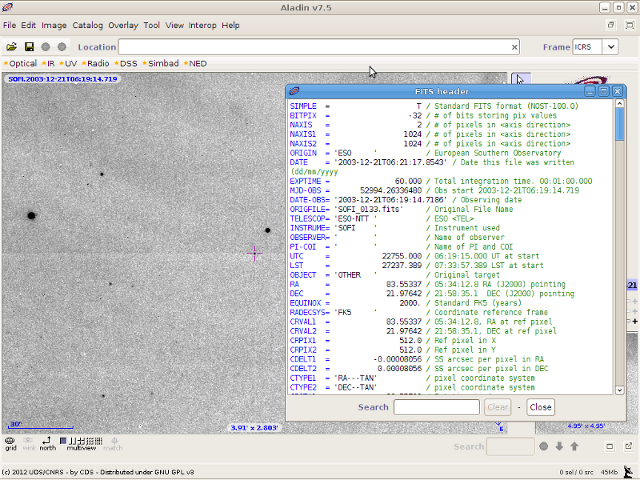
\includegraphics[width=11cm,height=8cm]{images/fits_header.png}
\caption{Viewing a FITS header in Aladin}
\end{figure}

% section flexible_image_transport_system (end)

\section{ObsTAP} % (fold)
\label{sec:obstap}


A data model is a description of the objects represented by a computer system with their properties and relationships, a logical model detailing the decomposition of a complex dataset into simpler elements, like a collection of concepts and rules used in defining data model. 

In 2011 IVOA proposed a new recommendation: Observation Data Model Core
Components~\cite{2011arXiv1111.1758L}
and its Implementation in the Table Access
Protocol~\cite{2010tap..irec.....D}.
That document was intended to be a description of the interface which integrated the data modeling and data access aspects in a single service.
In other words, ObsTAP is the combination of the TAP with the ObsCore data model.

\subsection{ObsCore Components Data Model}

Its aim is to get the generic data model for the metadata necessary to describe any astronomical observation. In the IVOA recommendation, the data are described using
% UML.
the Unified Modelling Language~\cite{Burkhardt:1997:UML} (UML).

\subsection{Table Access Protocol}

TAP defines a Web service for accessing tables containing astronomical catalogues. TAP is the protocol which underlies in the process of posing a query against a data source (or several data sources). The result of a query is a table, usually a VOTable.\footnote{Support for VOTable output is mandatory, while other formats may be available.}  

Queries which use TAP protocol can be made through several clients, like:
\begin{itemize}
\item TOPCAT\urlnote{http://www.star.bris.ac.uk/~mbt/topcat/}
\item TAPHandle\urlnote{http://saada.unistra.fr/taphandle/}
is a TAP client
 which operates fully within the Web browser
\item The TAP shell\urlnote{http://vo.ari.uni-heidelberg.de/soft/tapsh}, a command line interface to querying TAP servers, complete with metadata management and command line completion.
\item The GAVO VOTable library\urlnote{http://docs.g-vo.org/DaCHS/votable.html}, which allows embedding TAP queries in Python.
\end{itemize}

The types of queries implemented by TAP are:

\begin{itemize}
\item data queries, where the query result is directly the science data to be operated upon;
\item metadata queries, where the query result is metadata of the datasets, the archival service, or both; and
\item Virtual Observatory Support Interface (VOSI) queries, which provide information on the different TAP service capabilities.
\end{itemize}


TAP includes support for multiple query languages, including queries specified using the Astronomical Data Query Language (ADQL; see~\cite{2008adql.ivoav0910O}) and the Parameterised Query Language~\cite{IVOA-Data-Access-Layer-Working-Group:2009lr} (PQL, under development). Other query languages are also supported, and this mechanism allows developments outside the IVOA to be used without modifying the TAP specification. Finally, it also includes support for both synchronous and asynchronous queries. Special support is provided for spatially indexed queries using the spatial extensions in ADQL. 

Listing~\ref{lst:adqlsample} shows an ADQL sample query: a crossmatch between a user-uploaded catalog (\texttt{TAP\_UPLOAD.T1}), and
the Third US Naval Observatory CCD Astrograph Catalog\urlnote{http://www.usno.navy.mil/USNO/astrometry/optical-IR-prod/ucac} (UCAC3) % UCAC
catalog, compensating the fit for proper motion.

\begin{lstlisting}[float,language=SQL,caption={ADQL sample query: the results will be a crossmatch between a user-uploaded catalog, and the UCAC3 catalog, compensating the fit for proper motion.},label=lst:adqlsample]
SELECT 
 u.raj2000+d_alpha+d_pmalpha/cos(radians(u.dej2000))*(u.epoch-2000) AS ra_icrs,
 u.dej2000+d_delta+d_pmdelta*(u.epoch-2000) AS de_cicrs,
 u.pmra+d_pmalpha AS pmra_icrs,
 u.pmde+d_pmdelta AS pmde_icrs,
 u.*
FROM
  TAP_UPLOAD.T1 AS u
  JOIN ucac3.icrscorr AS c
  ON (c.alpha=FLOOR(u.raj2000)+0.5 and c.delta=FLOOR(u.dej2000)+0.5)
\end{lstlisting}

% section obstap (end)

\section{OpenCADC} % (fold)
\label{sec:opencadc}

OpenCADC (Canadian Astronomy Data Center) is a Virtual Observatory, used in ALMA Science Archive (for this reason is included in this chapter) tool which comprises several projects\footnote{We do not enumerate all of them here, for a full list, go to \url{https://code.google.com/p/opencadc/source/browse}}:

\subsection{Universal Worker Service}

The Universal Worker Service~\cite{2010uws..irec.....H} (UWS) 
standard defines a work
pattern 
that specifies
how to build asynchronous (as the client does not wait for each request to be fulfilled; even if the client disconnects from the service, activity is not aborted), stateful (the service remembers results of a previous activity), job-oriented services.

Job specification rules following the UWS pattern are written in the Job Description Language (JDL).

\begin{figure}[tb]
\centering
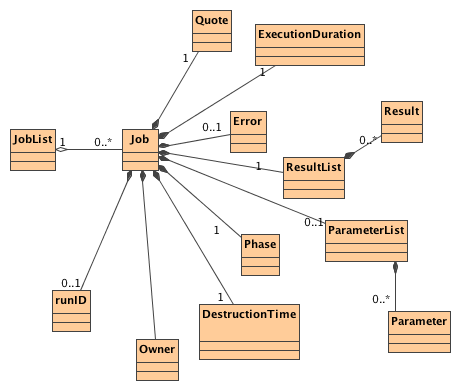
\includegraphics[width=11cm,height=8cm]{images/Class_Diagram__UWS__UWSObjects.png}
\caption{Class diagram representing UWS objects}
\end{figure}

When the execution starts, the job can adopt several states. The phases are the following:



\begin{figure}[tb]
\centering
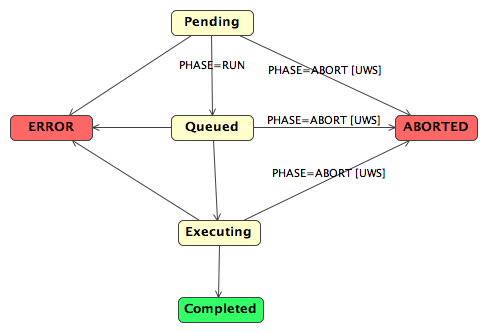
\includegraphics[width=11cm,height=8cm]{images/UWSStates.png}
\caption{Universal Worker Server Job states}
\end{figure}

Now, we make a subtle description of the structure of the code relating UWS in OpenCADC (the cadcUWS Library), the section of the code provides Job class and plugin architecture, servlet with UWS async and sync behaviour.

\subsubsection{JobManager}

Responsible for job control.

\subsubsection{JobPersistence}

In charge of storing and retrieving Job state.

\subsubsection{JobExecutor}

It executes every job in separated threads.

\subsubsection{JobRunner}

The code that actually executes the job.


\subsection{cadcTAP Library}

The cadcTAP library is responsible of async and sync queries, where QueryRunner implements JobRunner. It also contains TAP\_SCHEMA\footnote{TAP services try to be self-describing about what data they contain. They provide information on what tables they contain in special tables in TAP\_SCHEMA}
Data Definition Language\footnote{In RDBMS, the Data Definition Language is the language that allows for the creation of tables, fields, and data types.} (DDL) % DDL
statements and is used by query parser to validate table and column usage.

\subsubsection{TapQuery Interface}

It has a separate implementation for each LANG (e.g. \texttt{LANG=ADQL}) specified and processess the query to local SQL.

\subsubsection{SqlQuery}

When code states \texttt{LANG=SQL}, it implements TapQuery and fully navigates it (\texttt{FROM}, \texttt{WHERE} and \texttt{HAVING} clauses).

\subsubsection{AdqlQuery}

Same as before when \texttt{LANG=ADQL}.

\subsubsection{Plugins}

\begin{itemize}
\item UploadManager
\item TableWriter
\item FileStore
\end{itemize}


\subsubsection{QueryRunner}

It implements JobRunner and sets Job state, find DataSource and uses TapSchema, UploadManager, TapQuery and TableWriter.

% section opencadc (end)



% chapter the_virtual_observatory (end)
